\documentclass[12pt,titlepage]{article}

\setlength{\oddsidemargin}{0in}
\setlength{\evensidemargin}{0in}
\setlength{\textwidth}{6.5in}
%
\setlength{\textheight}{9in}
\setlength{\topmargin}{0in}
\setlength{\headsep}{0in}
\setlength{\topskip}{0in}
\setlength{\headheight}{0in}

\usepackage{graphicx}
\usepackage{times}
\usepackage[plainpages=false, colorlinks=true, anchorcolor=blue, linkcolor=blue, citecolor=blue, bookmarks=false, urlcolor=blue]
{hyperref}
\usepackage[square,comma,authoryear]{natbib}


\title{DOE Office of Science INCITE Project:\\
{\it Extreme-scale Simulation of Supernovae and Magnetars from Realistic Progenitors}\\
2020 Q1 Report}

\author{Principal Investigator:\\Sean M. Couch\\
  Michigan State University \vspace{0.1in}\\
  Co-Investigators: \\
  Andrew Christlieb (Michigan State University) \\
  Evan O'Connor (Stockholm University)\\
  Kuo-Chuan Pan (National Tsinghua University) \\
  Luke Roberts (Michigan State University) \\
  MacKenzie Warren (North Carolina State University) \\
}

\date{April 1, 2020}


\begin{document}


\maketitle


%%%%%%%%%%%%%%%%%%%%%%%%%%%%%%%%%
\section{Project Usage}

%%%%%%%%%%%%%%%%%%%


\begin{figure}
  \begin{tabular}{cc}
    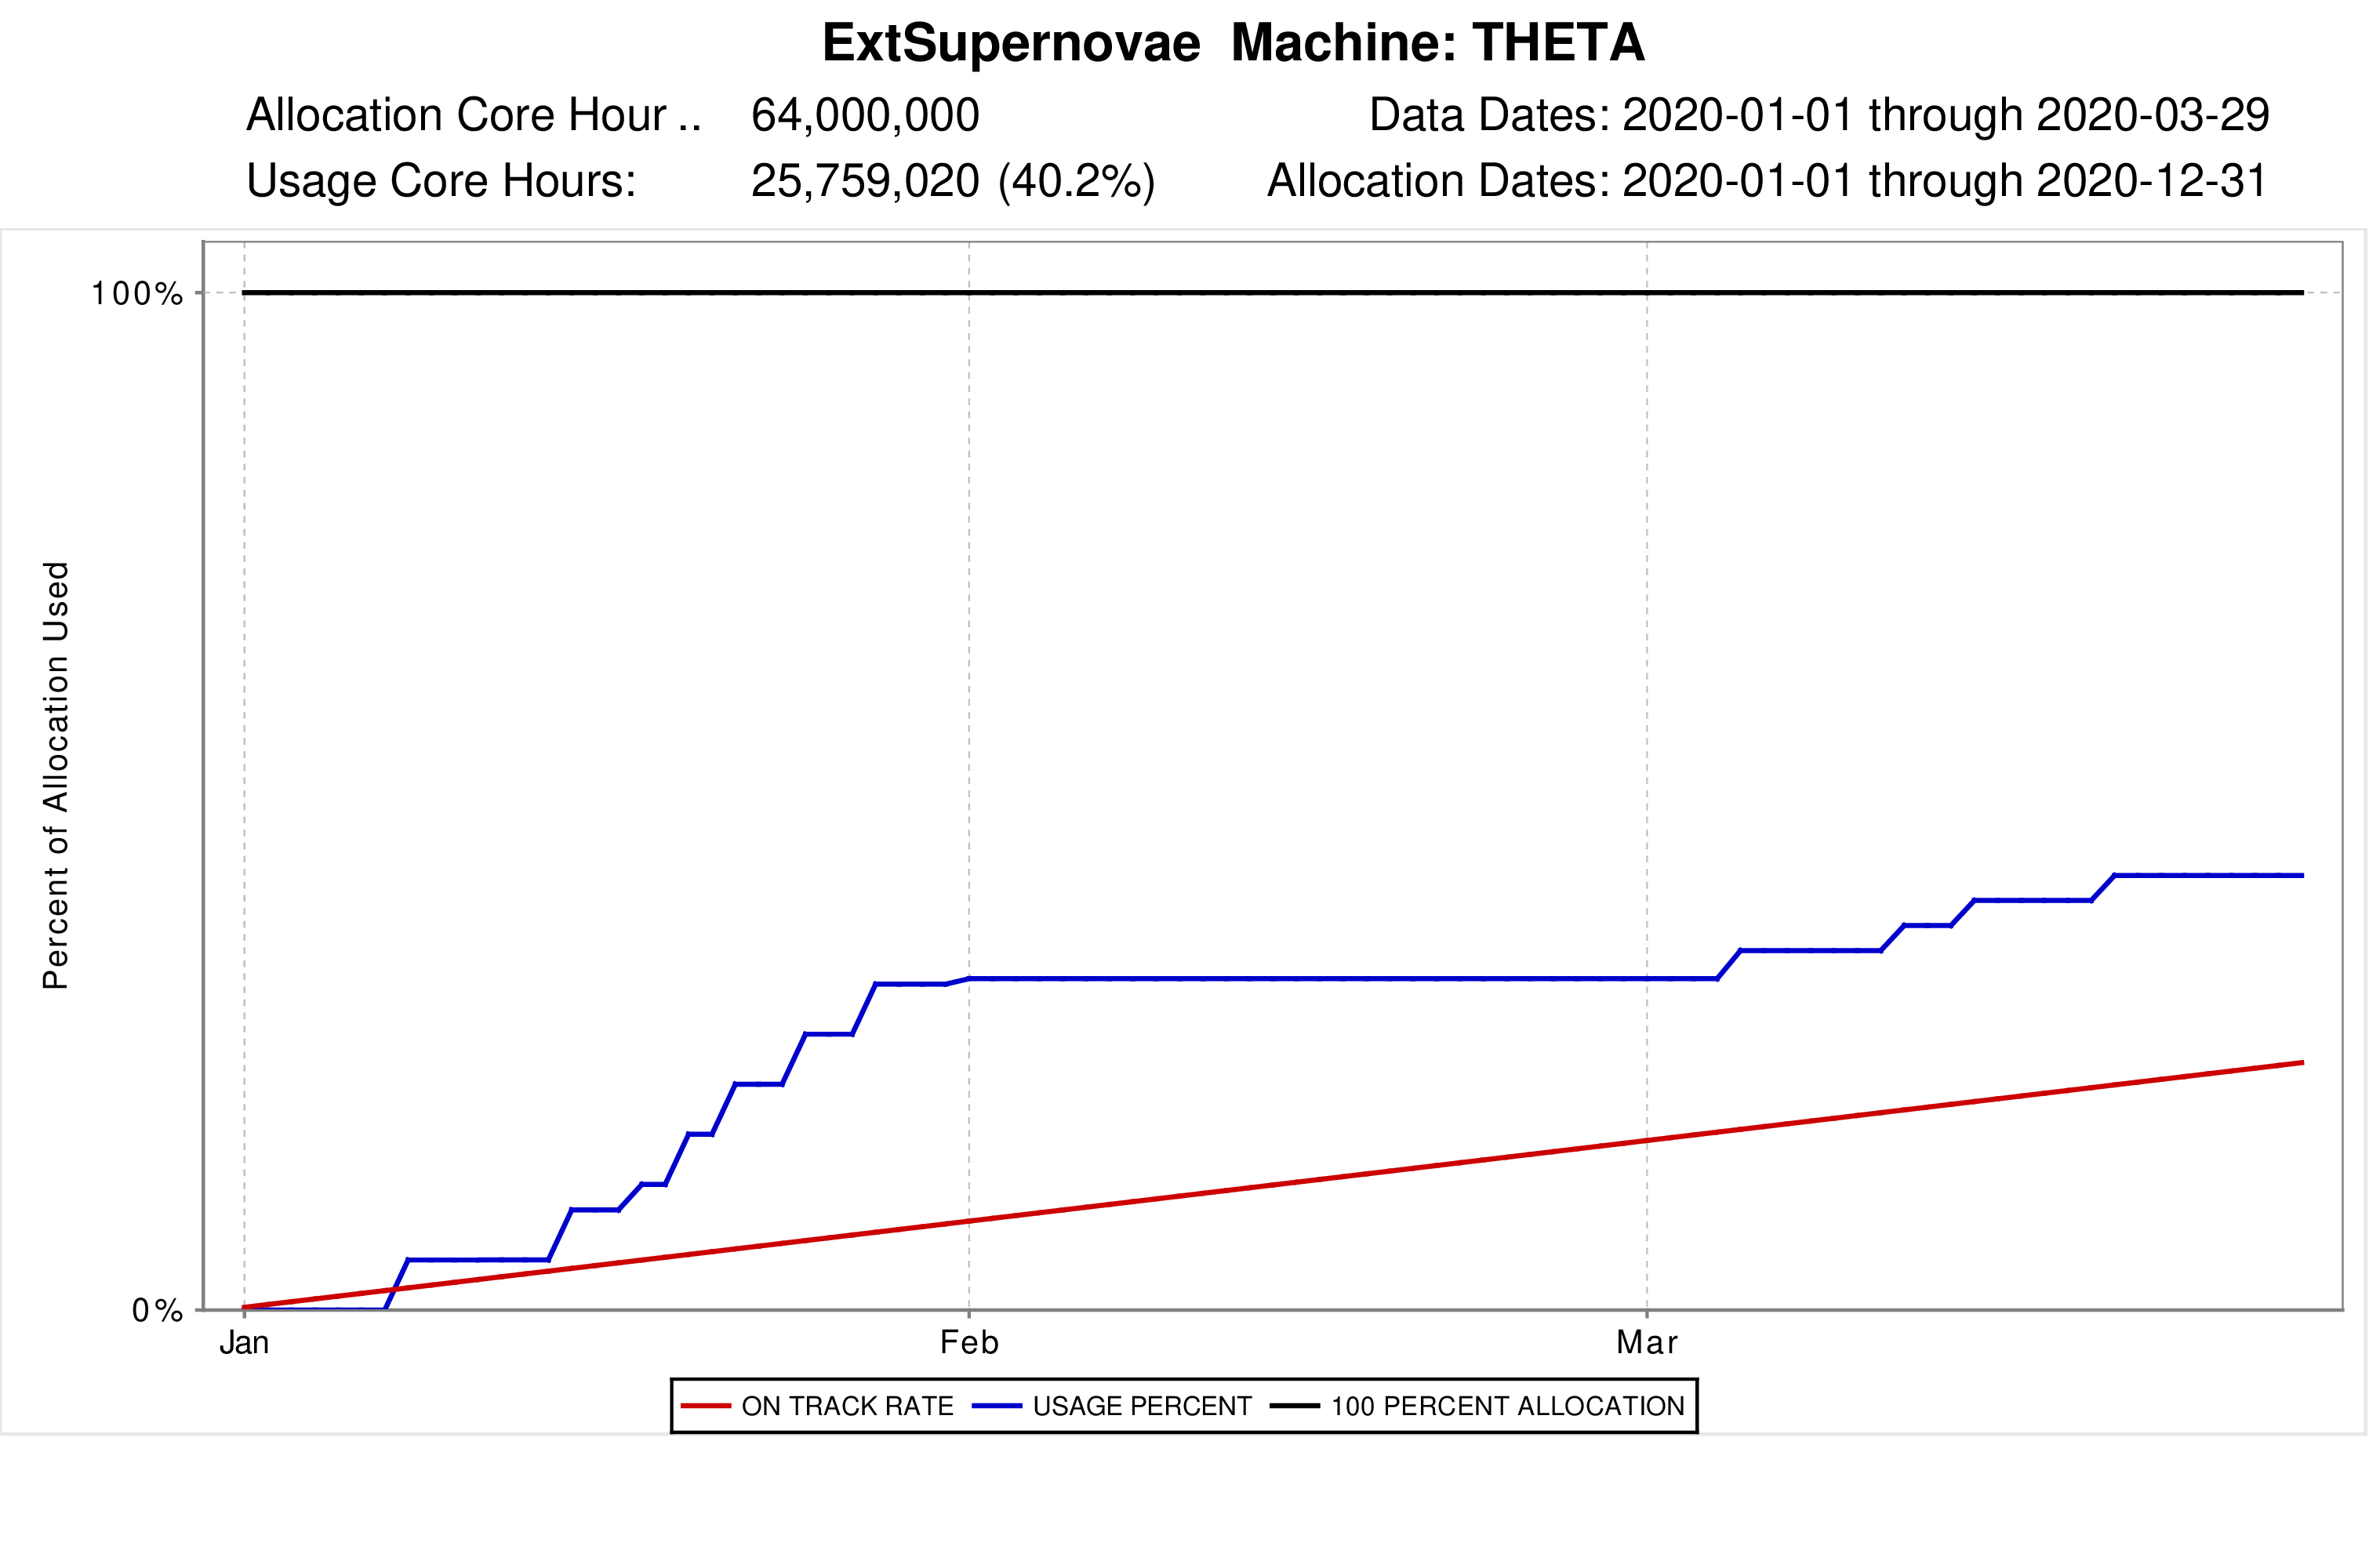
\includegraphics[width=3.25in]{on_track_graph}
    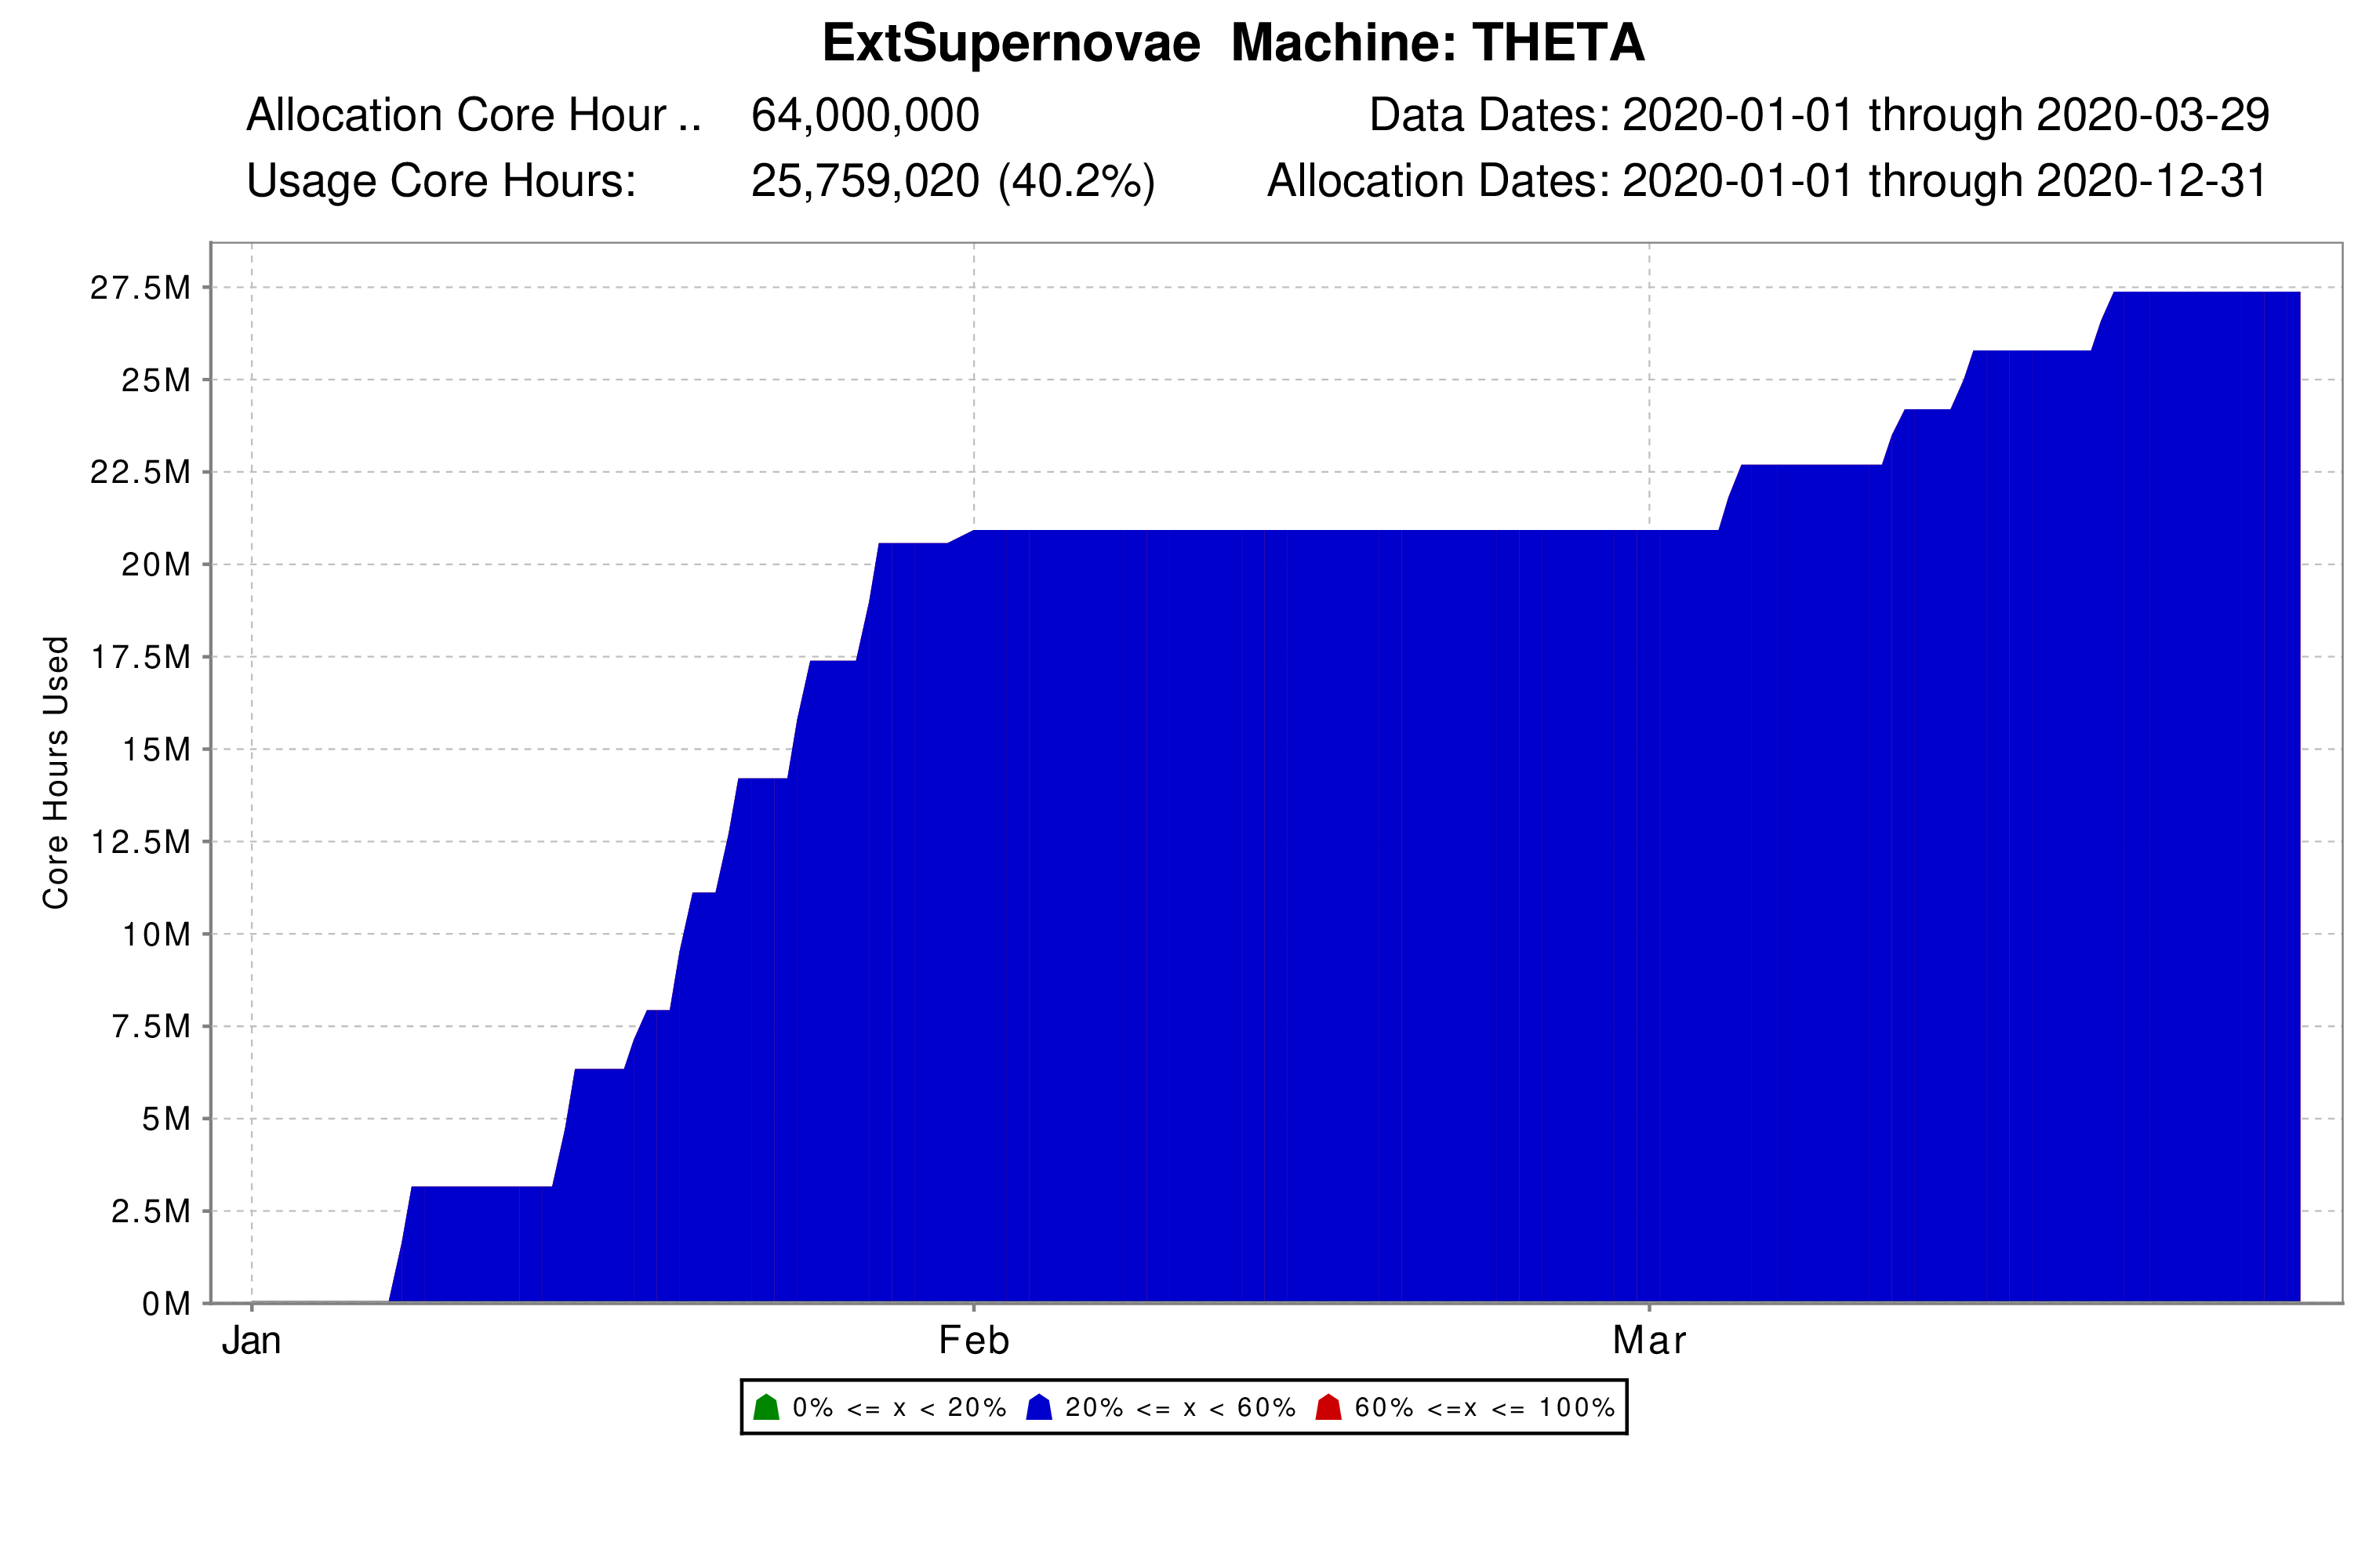
\includegraphics[width=3.25in]{categorized_hours_graph} 
  \end{tabular}
  \caption{Allocation usage.}
  \label{fig:usage}
\end{figure}

So far in 2020, we have expended 25.8M core-hours out of our allocation of 64M core-hours (40.2\% usage) on Theta. Firgure \ref{fig:usage} shows our usage so far. All of our usage so far has been at the Capability scale. 

%%%%%%%%%%%%%%%%%%%%%%%%%%%%%%%%%
\section{Report on Project Milestones}
%%%%%%%%%%%%%%%%%%%

Our milestones for Year 3, and corresponding progress, were:
\begin{enumerate}
    \item Adapt Spark-M1 to AMReX-based FLASH5 - This work is already underway as part of the {\it Exastar} Exascale Computing Project. Substantial progress has been made and we anticipate completing this milestone well before the end of Year 3.
    \item MHD CCSN Simulations Using 3D Progenitors - These simulations are deferred until suitable progenitors are available. This work will commence in Q2.
    \item Late-time CCSN simulation with 3D progenitors - This simulation ran at Capability scale on Theta. We made substantial progress on this simulation in Q1.
    \item Enhanced physics CCSN parameter study - This work will begin in Q2. 
\end{enumerate}



%%%%%%%%%%%%%%%%%%%%%%%%%%%%%%%%%
\section{Project Productivity}
%%%%%%%%%%%%%%%%%%%

\subsection{Primary}

\noindent {\bf Publications}
\begin{itemize}
    \item \href{https://ui.adsabs.harvard.edu/abs/2020arXiv200110434S/abstract}{``Equation of State and Progenitor Dependence of Stellar-Mass Black-Hole Formation''},  Schneider, A. S.; O'Connor, E.; Granqvist, E.; Betranhandy, A.; Couch, S. M., accepted to {\itshape Astrophysical Journal}, arXiv:2001.10434
\end{itemize}

\noindent {\bf Presentations}

\begin{itemize}
    \item ``Toward a Predictive Theory of Core-collapse Supernova Explosions,'' S.M. Couch, Embry Riddle Aeronautic University Physics and Astronomy Colloquium, March 2020.
\end{itemize}

% \subsubsection{Secondary}

% \begin{itemize}
%   \item Co-I and postdoc Kuo-Chuan Pan started a tenure-track faculty position at National Tsing Hua University in Taiwan.
%   \item Co-I and postdoc MacKenzie Warren won a prestigious NSF Postdoctoral Fellowship.
% \end{itemize}

\section{Center Feedback}

Our catalyst, Adrian Pope, has been extremely helpful.
He is now helping us tune our code for Theta.


\section{Code Description and Characterization}

\texttt{FLASH} is a highly capable, fully modular, extensible,
community code that is widely used in astrophysics, cosmology, fluid
dynamics, and plasma physics, and other fields.  The capabilities of
the FLASH code include adaptive mesh refinement (AMR), several
self-gravity solvers, an advection-diffusion-reaction (ADR) flame
model, an accurate and detailed treatment of nuclear burning, and a
sophisticated two-moment neutrino transport scheme based on an
explicit hyperbolic solver.  The neutrino interactions are included
through the open-source neutrino interaction library
\texttt{NuLib}. We have enhanced the
performance of the two-moment neutrino transport scheme significantly
as well as upgraded the transport to now include full velocity and
gravitational red-shift dependence in the evolution equations.

\texttt{FLASH} is written in modern Fortran, with some utility
functions written in C, and a build system written in Python.  It
requires MPI library support, and either HDF5 or P-NetCDF for I/O.
Additional mathematical software, such as \texttt{Hypre}, may be
required to configure \texttt{FLASH} for particular simulations.

Algorithm classes used within \texttt{FLASH} include Sparse Linear
Algebra solvers, FFT, active and passive particles, structured grids,
and AMR.



\end{document}
